%\documentclass[12pt, handout]{beamer}
\documentclass[12pt]{beamer}

\usepackage{cmap}
\usetheme{Madrid}
\usepackage[utf8]{inputenc}
\usepackage[russian]{babel}
\usepackage[OT1]{fontenc}
\usepackage{amsmath}
\usepackage{amsfonts}
\usepackage{amssymb}
\usepackage{graphicx}
\usepackage{listings}
\usepackage{comment}

\author{Игорь Рязанцев}
\title{Введение в Python}
\institute{Лекция 01}
\date{2021г.}

%\setbeamercovered{transparent} 
\setbeamertemplate{navigation symbols}{} 
%\logo{} 
%\institute{} 
%\date{} 
%\subject{} 

\begin{document}

\begin{frame}
\titlepage
\end{frame}

\begin{frame}{План мини-курса}
\begin{itemize}
\item \textbf{Лекция 01. Введение в Python}
	\begin{itemize}
	\item Переменные в Python
	\item Кортежи
	\item Списки	
	\item Циклы	
	\end{itemize}
\item \textbf{Лекция 02. Функции и объекты} \href{python_mini-course_02.pdf}{\beamerbutton{Открыть}}
	\begin{itemize}
	\item Функции
	\item Объектно-ориентированное программирование	
	\end{itemize}
\item \textbf{Лекция 03. Файлы и ввод-вывод в Python} \href{python_mini-course_03.pdf}{\beamerbutton{Открыть}}
	\begin{itemize}
	\item Понятия файлов (текстовые и бинарные)
	\item Ввод-вывод данных
	\end{itemize}
\item \textbf{Лекция 04. Построение графиков} \href{python_mini-course_04.pdf}{\beamerbutton{Открыть}}
	\begin{itemize}
	\item Вывод графиков функций 
	\item Математическая библиотека numpy
	\end{itemize}
\end{itemize}
\end{frame}


\begin{frame}{Что есть Python?}
\textbf{Python} -- высокоуровневый язык программирования общего назначения с динамической строгой типизацией и автоматическим управлением памятью 
\center{
\includegraphics[scale=0.1]{image/python.jpg}}
\end{frame}

\begin{frame}{Зачем изучать Python?}
\textbf{Зачем изучать Python, если вы не программист?}
\vspace{0.5cm}
\begin{itemize}
\item Python – легкий язык программирования;
\item Научит вас думать;
\item Сделает вас более самодостаточным;
\item Знание Python облегчит коммуникацию с разработчиками;
\item Поможет визуализировать данные;
\item Позволит автоматизировать повторяющиеся задачи;
\item Рынок вас ждет...
\end{itemize}
\end{frame}

\begin{frame}{TIOBE Index for May 2021}
\center{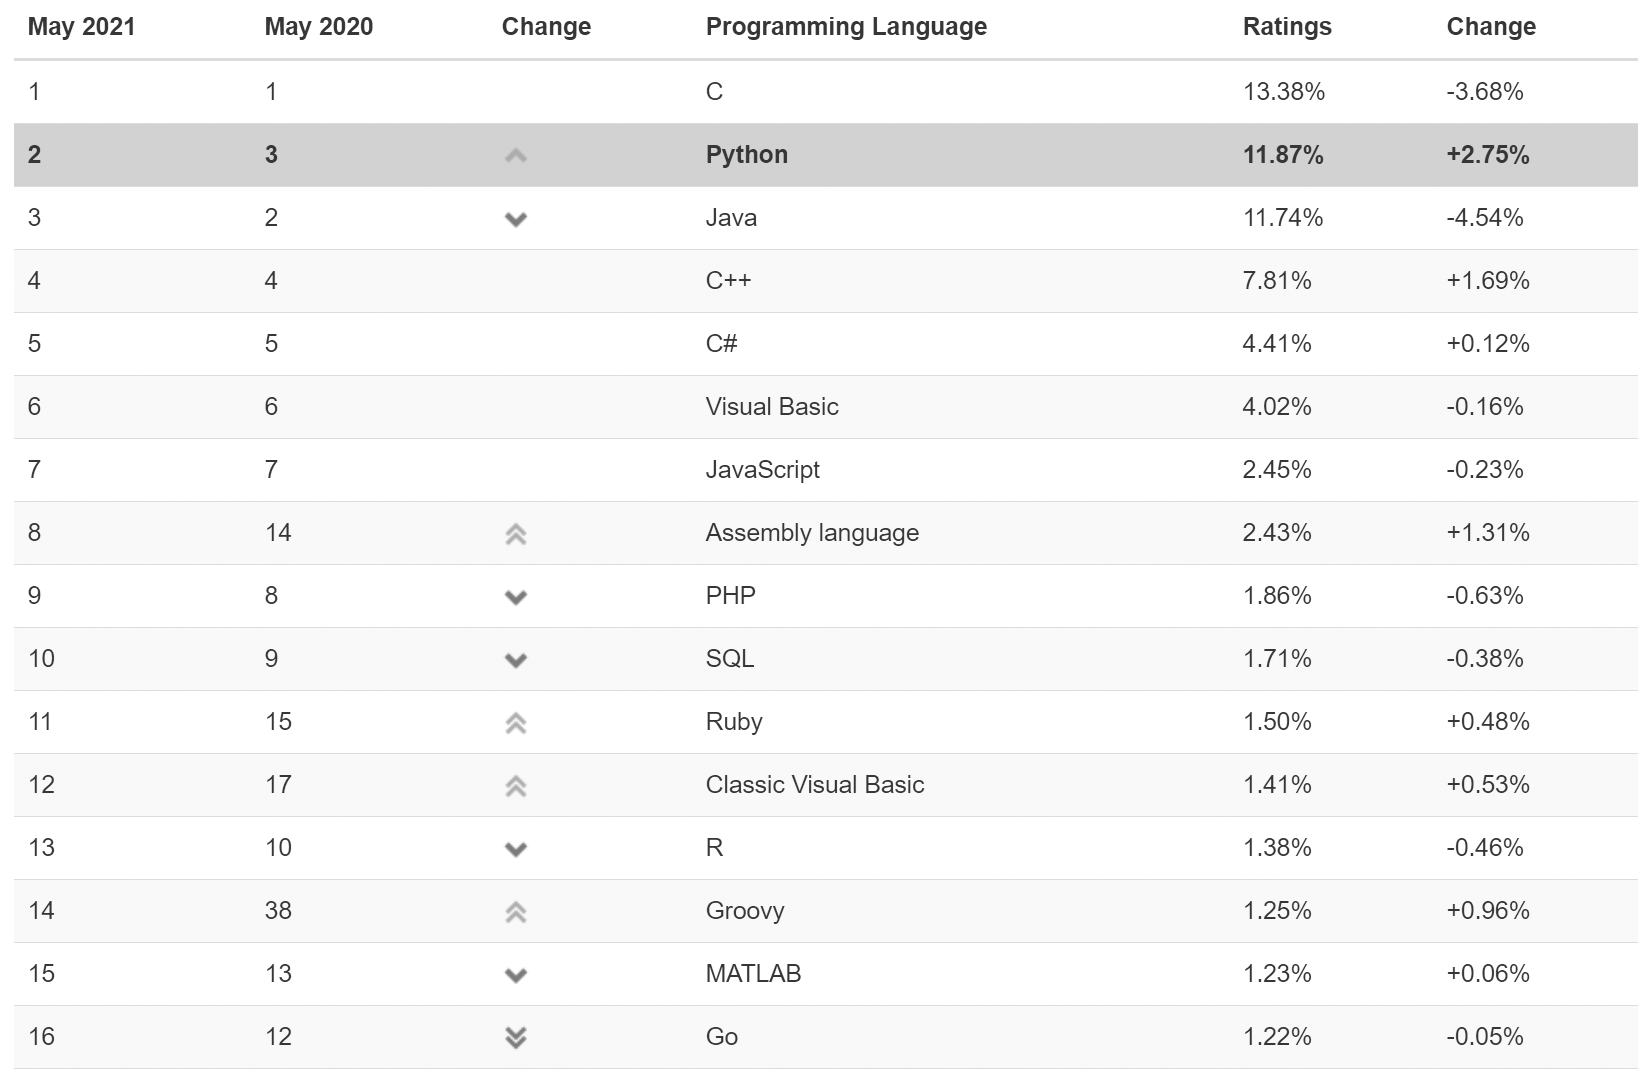
\includegraphics[scale=0.2]{image/TIOBE_Index.PNG}} 
\end{frame}

\begin{frame}{TIOBE Index for May 2021}
\center{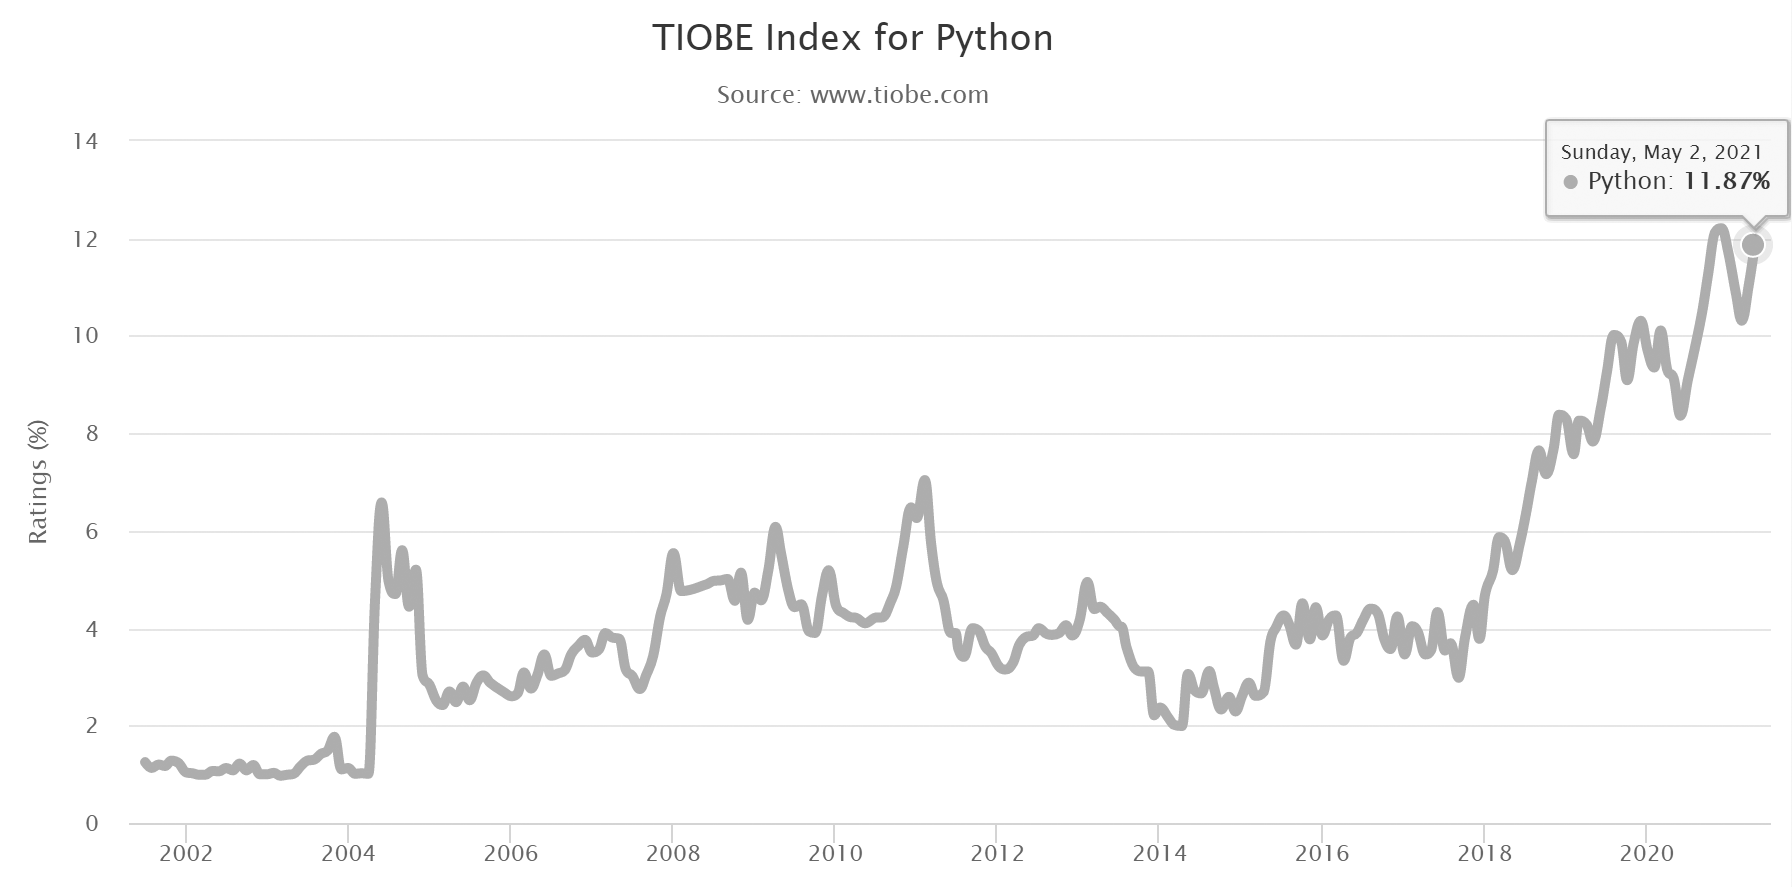
\includegraphics[scale=0.2]{image/TIOBE_Index_python.PNG}} 
\end{frame}

\begin{comment}
	\begin{frame}{hh.ru}
		\center{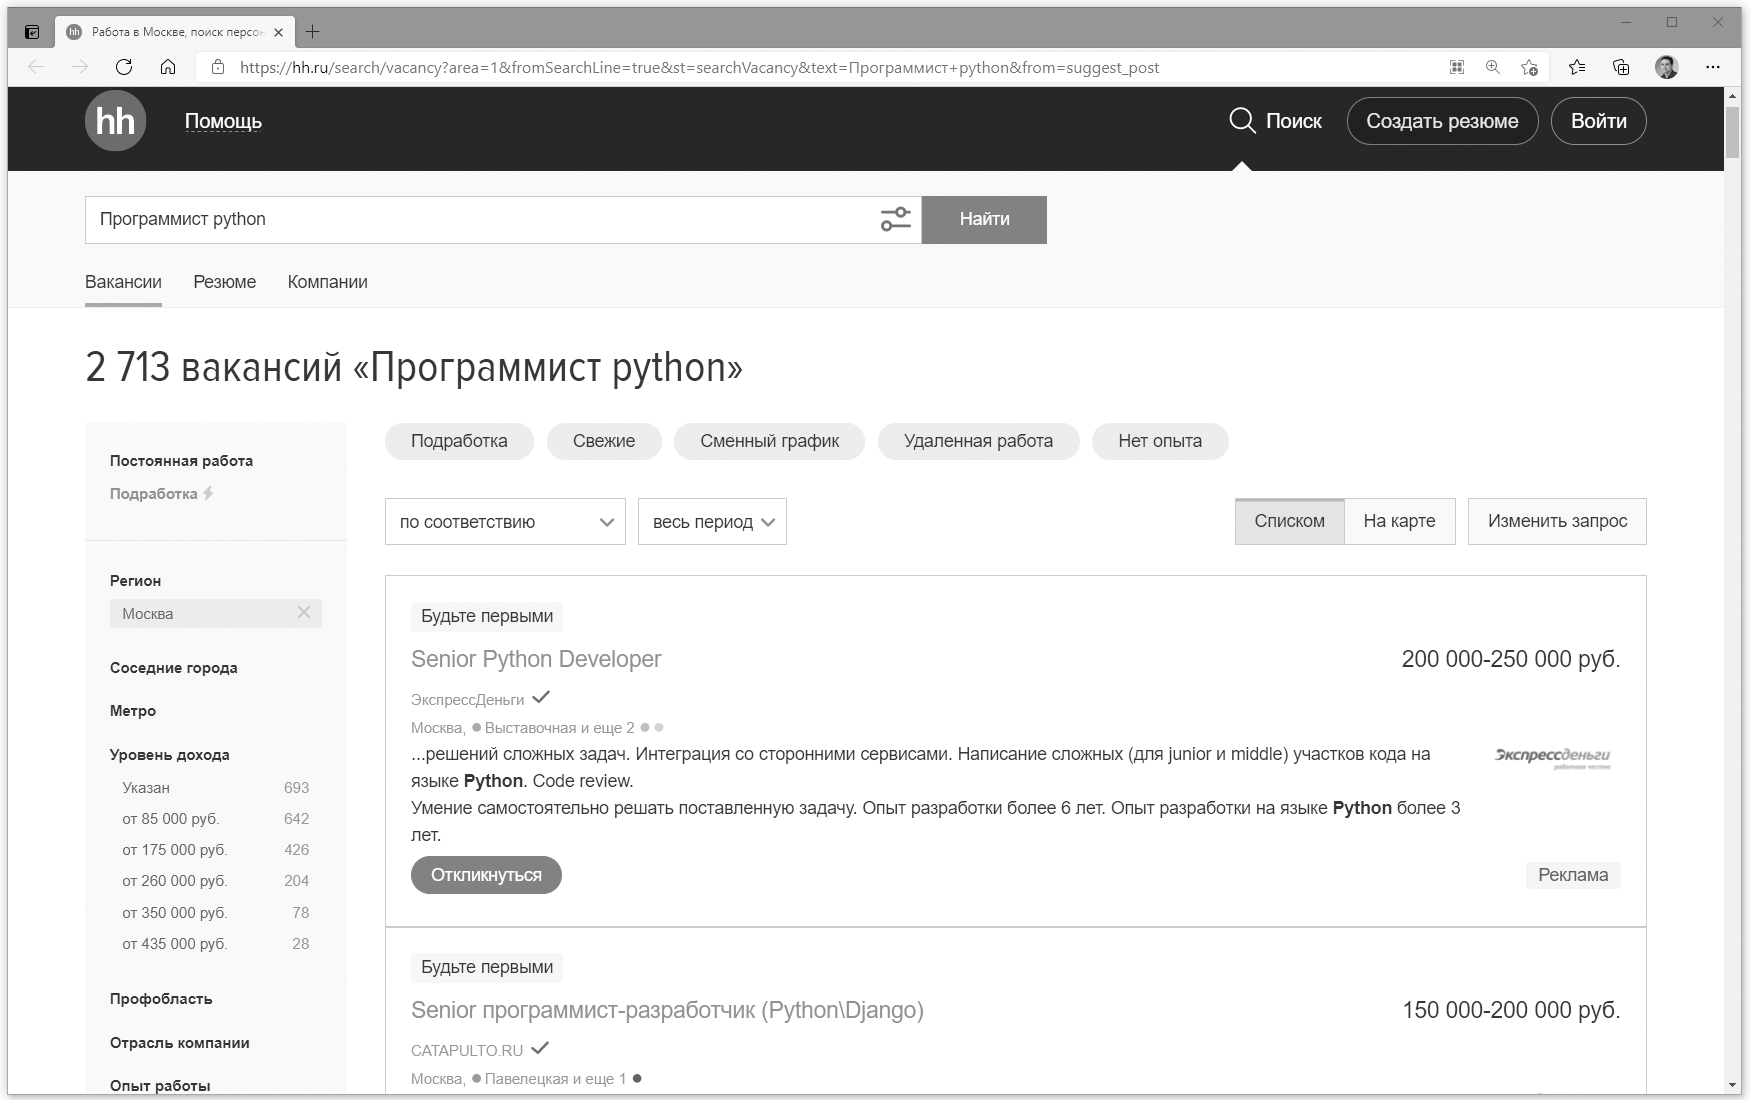
\includegraphics[scale=0.2]{image/hh_ru.PNG}} 
	\end{frame}
\end{comment}

\begin{frame}{История Python}
\begin{columns}[onlytextwidth,T]
    \column{30mm}
	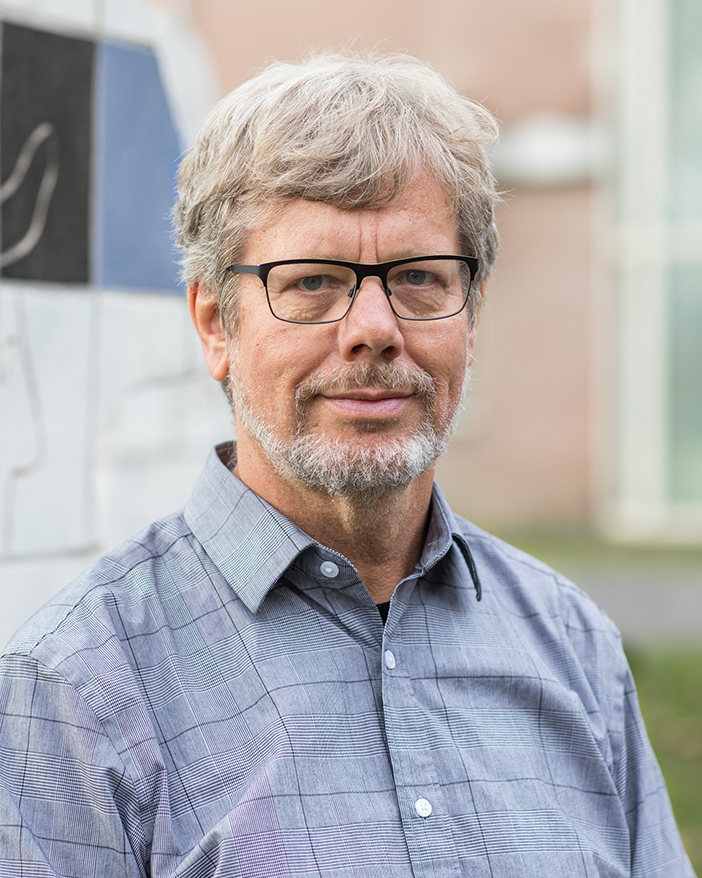
\includegraphics[scale=0.7]{image/Guido_van_Rossum.jpg}
    \column{\dimexpr\linewidth-30mm-20mm}
    Python начал разрабатывать в конце 80-x годов \textbf{Гвидо ван Россумом}. Python назван в честь телешоу <<Летающий цирк Монти Пайтона>> \\
    \vspace{0.3cm}
    Даты выпуска основных версий:
	\begin{itemize}
    	\item Python 1.0 — январь 1994 года
    	\item Python 2.0 — 16 октября 2000 года
    	\item Python 3.0 — 3 декабря 2008 года   	    	
    \end{itemize}           
    \vspace{0.3cm}
    Python 2.x и Python 3.x не совместимы!
    \end{columns}  
\end{frame}


\begin{frame}{Области применения Python}
\textbf{Что можно разрабатывать на Python?}
\vspace{0.5cm}
\begin{itemize}
\item Web-сайты;
\item Скрипты, утилиты, т.к. Python -- интерпретируемый язык программирования;
\item Программы с графическим интерфейсом;
\item Arduino, Raspberry Pi, Интернет вещей и умный дом;
\item Big-data;
\item Нейронные сети;
\item и т.п.
\end{itemize}
\end{frame}

\begin{frame}{Python}
\textbf{Плюсы Python:}
\vspace{0.5cm}
\begin{itemize}
\item Легкий для обучения;
\item Легко читаемый;
\item Широкая стандартная библиотека;
\item Наличие интерактивного режима;
\item Портативность;
\item Расширяемость;
\item Работа с базами данных;
\item Создание GUI;
\item Объектно-ориентированный язык программирования.
\end{itemize}
\end{frame}

\begin{frame}{Python}
\textbf{Недостатки Python\footnote{в сравнении с кодом на компилируемых языках, т.к. C/C++}:}
\vspace{0.5cm}
\begin{itemize}
\item Низкая скорость работы;
\item Интерпретируемый язык программирования.
\end{itemize}
\end{frame}

\begin{frame}{Python}
\textbf{Сайты написанные на Python:}
\vspace{0.5cm}
\begin{itemize}
\item YouTube
\item Instagram
\item Google Search
\item DropBox
\item Spotify
\item Netflix
\item и многие другие ...
\end{itemize}
\end{frame}

\begin{frame}{Установка Python}
\center{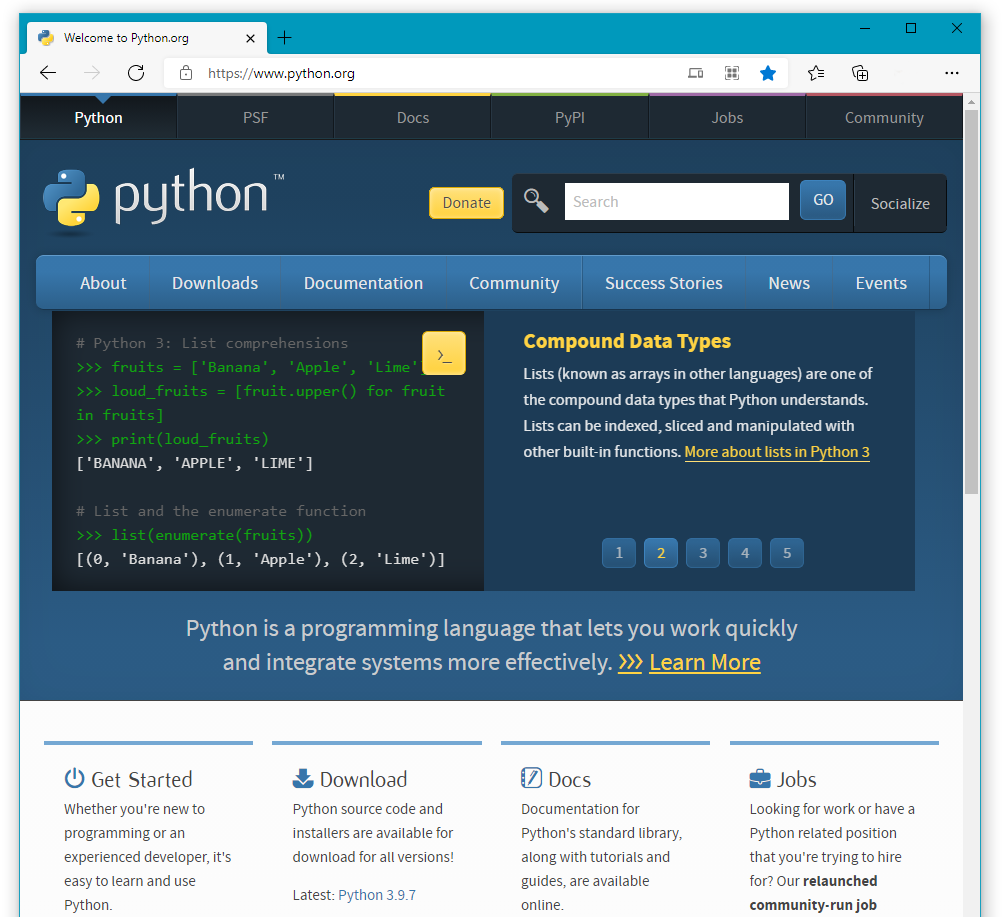
\includegraphics[scale=0.32]{image/www_pathon_org.png}}
\end{frame}

\begin{frame}{Python}
\textbf{IDE (интегрированная среда разработки):}
\vspace{0.5cm}
\begin{itemize}
\item VSCode \href{https://code.visualstudio.com/}{\beamerbutton{Открыть}}
\item PyCharm  \href{https://www.jetbrains.com/pycharm/}{\beamerbutton{Открыть}}
\item Google Search
\item Блокнот и другие
\end{itemize}
\end{frame}

\begin{frame}{Python Programming Interpreter}
\vspace{0.9cm}
\begin{center}
	\begin{tabular}{ccc}
		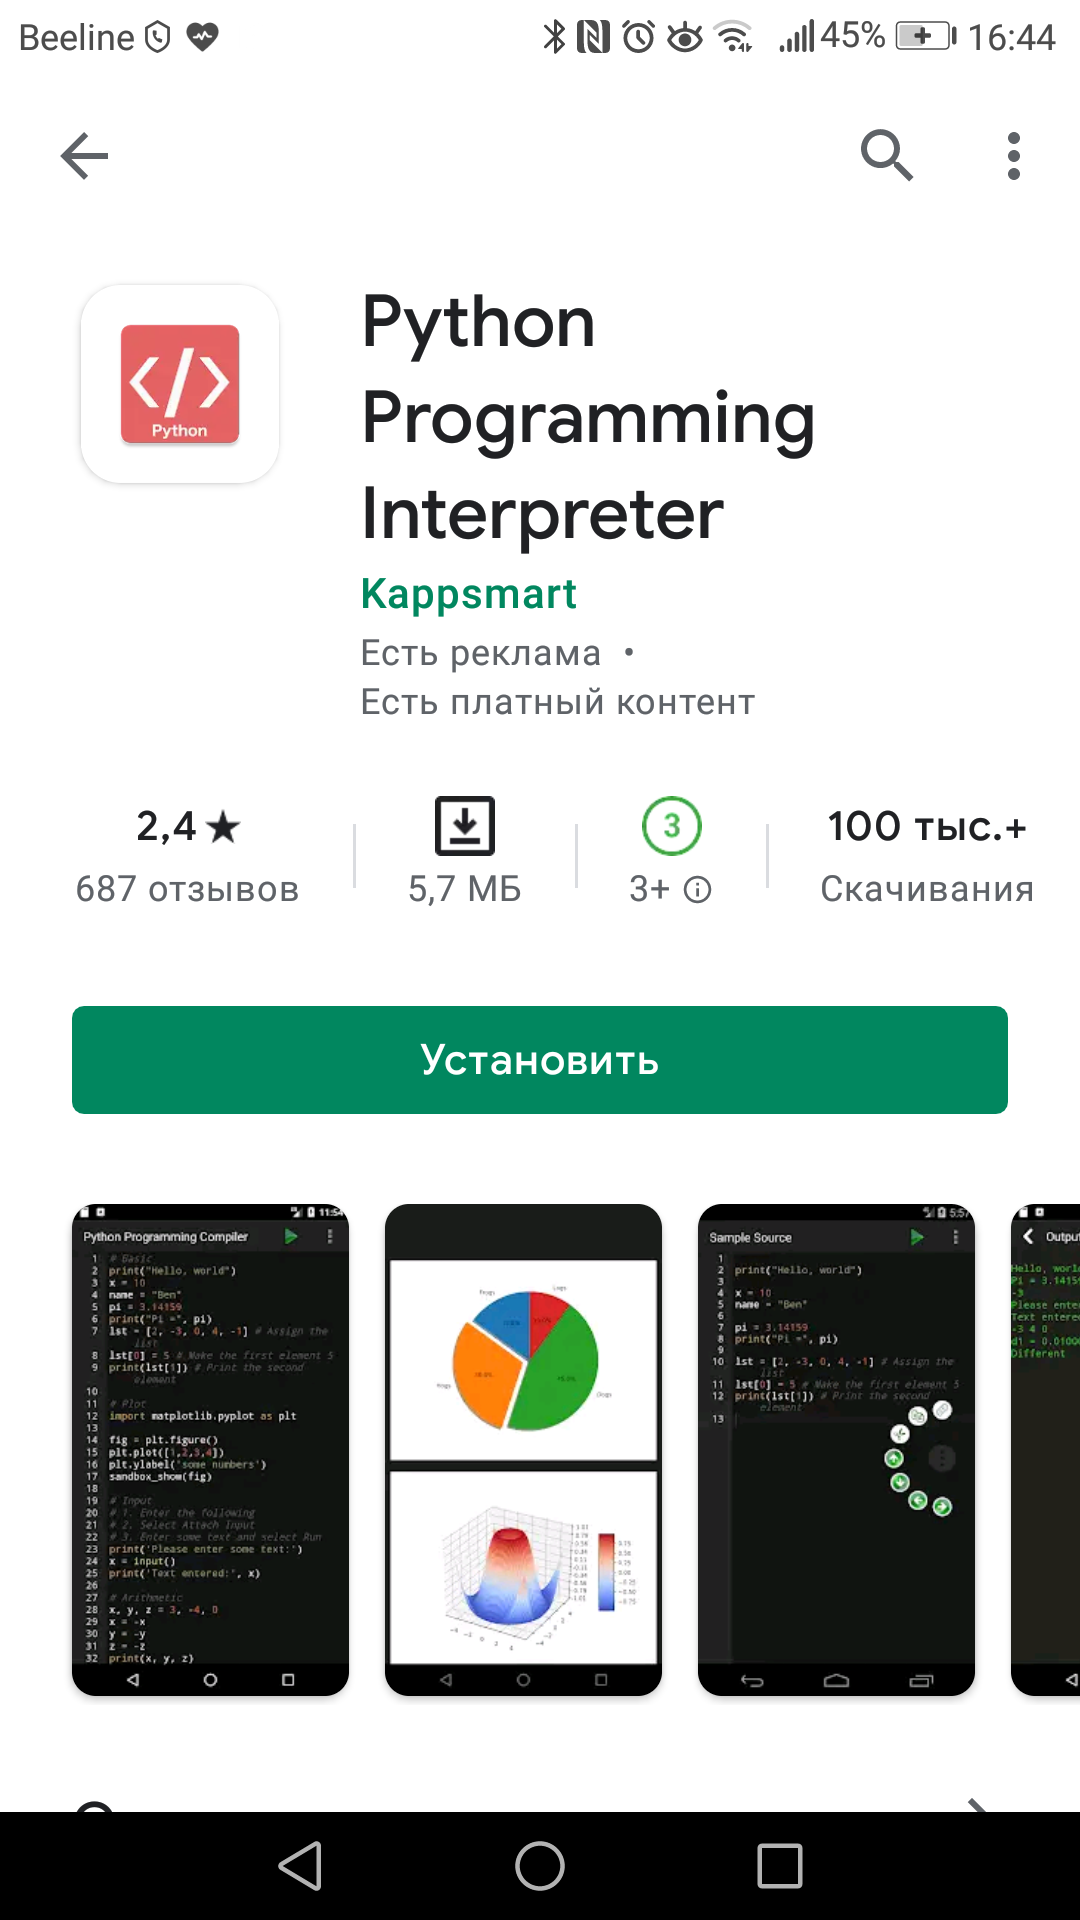
\includegraphics[scale=0.083]{image/interpreter_01.PNG} & 		
		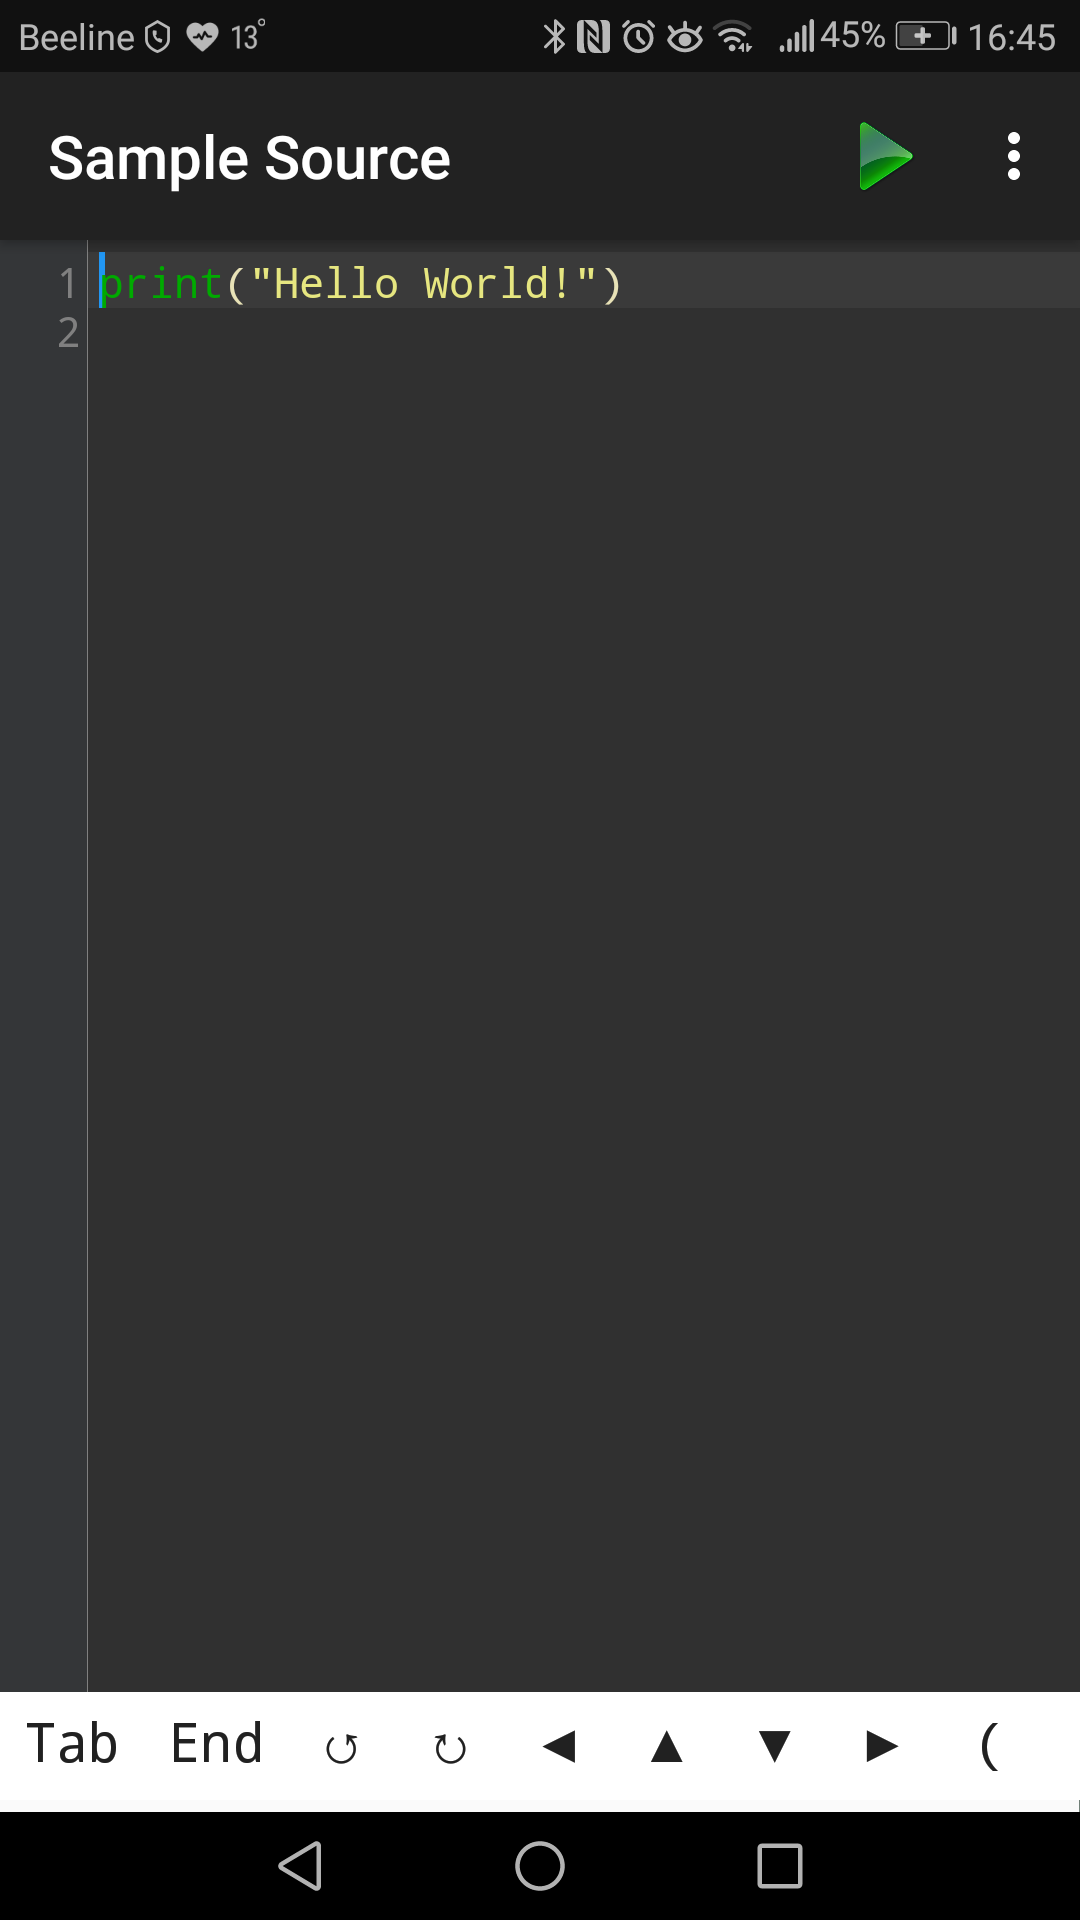
\includegraphics[scale=0.083]{image/interpreter_02.PNG} & 
		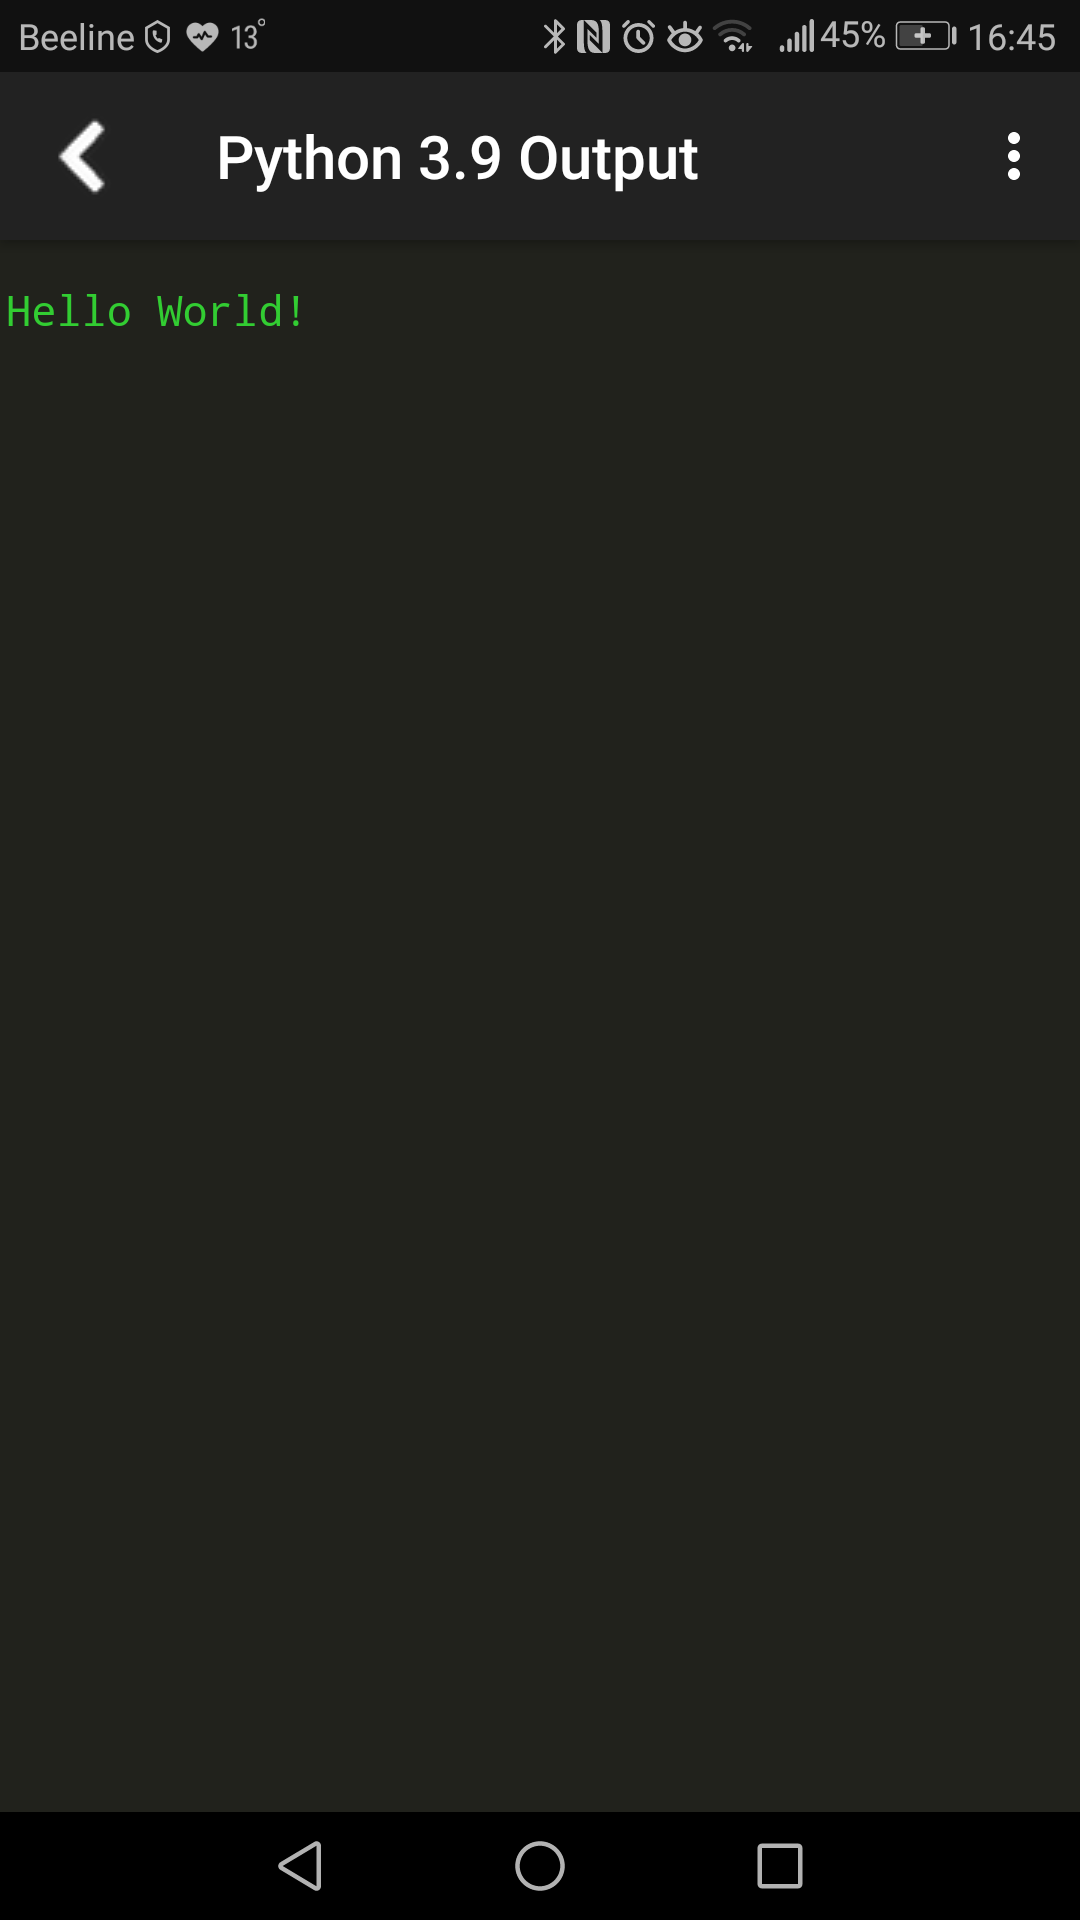
\includegraphics[scale=0.083]{image/interpreter_03.PNG} \\ 
	\end{tabular} \\
	\vspace{0.5cm}
	\href{https://play.google.com/store/apps/details?id=com.krazeapps.pythonprogrammingcompiler}{\beamerbutton{Открыть}}
\end{center}
\end{frame}

\begin{frame}{PyCharm}
\center{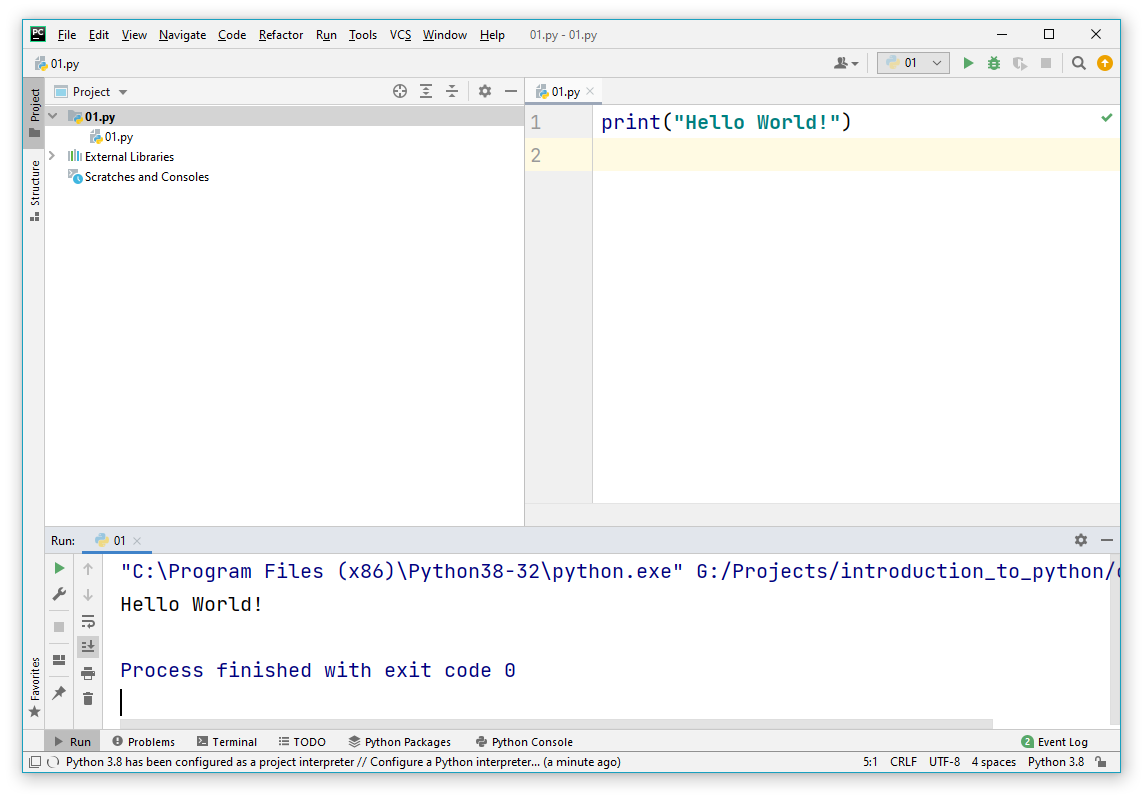
\includegraphics[scale=0.32]{image/PyCharm.png}} \\
\href{https://www.jetbrains.com/pycharm/}{\beamerbutton{Загрузить}}
\end{frame}


\begin{frame}[t]{Оглавление}
\tableofcontents[part=1]
\end{frame}

%\begin{frame}[t]{Оглавление}
%\tableofcontents
%\end{frame}

\part{1}
\section{Hello World!}
\begin{frame}{Hello World!}
\textbf{\# Первая программа, функция print}
\lstinputlisting[language=Python]{code/01.py}
\vspace{0.5cm}
\# или
\lstinputlisting[language=Python]{code/01_1.py}
\end{frame}


\section{Переменные в Python}
\begin{frame}{Переменные}
\textbf{\# Вывод значений переменной, вариант 1}
\lstinputlisting[language=Python]{code/02.py}
\vspace{0.5cm}
\textbf{\# s -- для строковых переменных}

\textbf{\# d -- для целых чисел}\

\textbf{\# f -- для чисел с плавающей запятой}
\end{frame}


\begin{frame}{Форматирование str.format}
\textbf{\# Вариант 2 (str.format)}
\lstinputlisting[language=Python]{code/03.py}
\vspace{0.5cm}
\# вывод нескольких значений переменных
\lstinputlisting[language=Python]{code/04.py}
\end{frame}

\begin{frame}{Форматирование str.format}
\vspace{0.5cm}
\lstinputlisting[language=Python]{code/04.py}
\end{frame}


\section{Кортежи}
\begin{frame}{Кортежи tuple()}
\textbf{\# Кортежи -- упорядоченная последовательность \\ \# произвольных объектов, типы которых могут \\ \# различаться}
\vspace{0.5cm}
\lstinputlisting[language=Python]{code/05.py}
\vspace{0.5cm}
\end{frame}


\section{Списки}
\begin{frame}{Списки list()}
\textbf{\# Список -- это тоже упорядоченная последовательность \\ \# произвольных объектов, типы которых могут \\ \# различаться}
\vspace{0.5cm}
\lstinputlisting[language=Python]{code/06.py}
\vspace{0.5cm}
\end{frame}


\section{Циклы}
\begin{frame}{Цикл for}
\textbf{\# В Python вложенные инструкции объединяются в блоки по величине отступов. Отступ может быть любым, главное, чтобы в пределах одного вложенного блока отступ был одинаков.\footnote{используйте 4 пробела} }
\vspace{0.5cm}
\lstinputlisting[language=Python]{code/06_1.py}
\vspace{0.5cm}
\end{frame}


\begin{frame}{Цикл for. Функция range()}
\textbf{\# Функция \textbf{range()} упрощает построение числовых последовательностей.}
\vspace{0.5cm}
\lstinputlisting[language=Python]{code/07.py}
\vspace{0.5cm}
Результат: \\
1 \\
2 \\
3 \\
4 \\
\end{frame}


\begin{frame}{Операции со списком}
\textbf{\# append() -- добавить элемент в конец} 
\vspace{0.5cm}
\lstinputlisting[language=Python]{code/08.py}
\vspace{0.5cm}
Результат: \\
1 \\
2 \\
3 \\
4 \\
5 \\
\end{frame}


\begin{frame}{Операции со списком}
\textbf{\# insert(позиция, элемент) -- добавить элемент в указанную позицию} 
\vspace{0.5cm}
\lstinputlisting[language=Python]{code/09.py}
\vspace{0.5cm}
Результат: \\
0 \\
1 \\
2 \\
3 \\
4 \\
\end{frame}


\begin{frame}{Операции со списком}
\textbf{\# remove(элемент) -- удаление элемента по значению} \\
\textbf{\# pop(позиция) -- удаление элемента по индексу\footnote{Значение индекса в списке начинается с 0}} 
\vspace{0.5cm}
\lstinputlisting[language=Python]{code/10.py}
\vspace{0.5cm}
Результат: \\
1 \\
3 \\
\end{frame}


\begin{frame}{Операции со списком}
\textbf{\# sort() -- сортировка элементов списка} \\
\textbf{\# sort(reverse=True) -- сортировка в обратном порядке} 
\vspace{0.5cm}
\lstinputlisting[language=Python]{code/11.py}
\vspace{0.5cm}
Результат: \\
1 \\
2 \\
3 \\
4 \\
\end{frame}


\begin{frame}{Тестовое задание}
\textbf{\# Необходимо вывести имена в алфавитном порядке} 
\vspace{0.5cm}
\lstinputlisting[language=Python]{code/12.py}
\vspace{0.5cm}
Результат: \\
Calvin \\
Henry \\
Sam \\
\end{frame}


\begin{frame}{Тестовое задание}
\textbf{\# Вариант 1} 
\vspace{0.5cm}
\lstinputlisting[language=Python]{code/13.py}
\vspace{0.5cm}
Результат: \\
Calvin \\
Henry \\
Sam \\
\end{frame}


\begin{frame}{Тестовое задание}
\textbf{\# Вариант 2.} 
\vspace{0.5cm}
\lstinputlisting[language=Python]{code/14.py}
\vspace{0.5cm}
Результат: \\
Calvin \\
Henry \\
Sam \\
\end{frame}


\section{Оператор if}
\begin{frame}{Оператор if}
\textbf{\# Оператор условного перехода}
\vspace{0.5cm}
\lstinputlisting[language=Python]{code/15.py}
\vspace{0.5cm}
Результат: \\
Audi \\
BMW \\
Toyota \\
\end{frame}


\begin{frame}{Оператор if}
В \textbf{if} центральное место занимает выражение, результатом которого является логическая истина \textbf{(True)} или логическая ложь \textbf{(False)}; это выражение называется \textit{условием}.\\
\vspace{0.5cm}
\textbf{\# Общая форма записи:}
\vspace{0.5cm}
\lstinputlisting[language=Python]{code/16.py}
\vspace{0.5cm}
\end{frame}


\begin{frame}{Оператор if}
\begin{tabular}{|c|c|}
\hline 
== & равно \\ 
\hline 
> & больше \\ 
\hline 
>= & больше или равно \\ 
\hline 
<= & меньше или равно \\ 
\hline 
< & меньше \\ 
\hline 
\end{tabular} 
\par
\vspace{0.5cm}
\lstinputlisting[language=Python]{code/16_1.py}
\end{frame}


\begin{frame}{Тестовое задание}
\textbf{\# Необходимо вывести наименование светильника c наибольшим световым потоком и наименьшей потребляемой мощностью} 
\vspace{0.5cm}
\lstinputlisting[language=Python]{code/17.py}
\vspace{0.5cm}
\end{frame}


\part{2}
\begin{frame}[t]{Вопросы}
\vspace{0.7cm}
\center{
\includegraphics[scale=0.3]{image/questions.jpg}} \\
\end{frame}

\end{document}